% Conference-native artwork: figures are NOT scaled-down general-paper plates.
\newcommand{\FableFigure}{
\begin{figure*}[!t]
\centering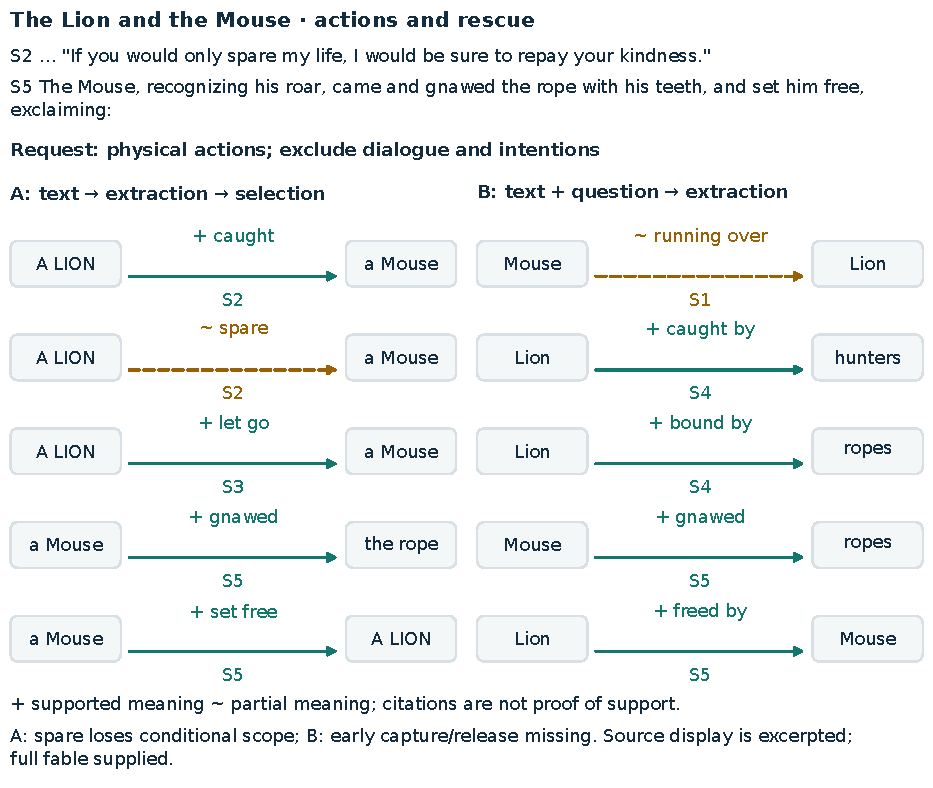
\includegraphics[width=\textwidth]{figures/fable.pdf}
\caption{Fable actions from pre-extract/select (A) and independent contextual extraction (B). + indicates supported meaning and $\sim$ partial meaning. Display: five of eight A records and all five B records. A's awakening, hunter capture and rope binding are omitted only from display. All predictions remain scored. Executed question: \FableQuestion\ Source display excerpts S2 and S5 from the complete supplied fable. The spare edge loses conditional scope and retains the misspelled key \texttt{valid until}. B loses the face-specific running endpoint and omits the early capture/release. Other displayed qualifications are null. Assessments are Codex-authored.}
\label{fig:fable}
\end{figure*}}
\newcommand{\HarborFigure}{
\begin{figure*}[!t]
\centering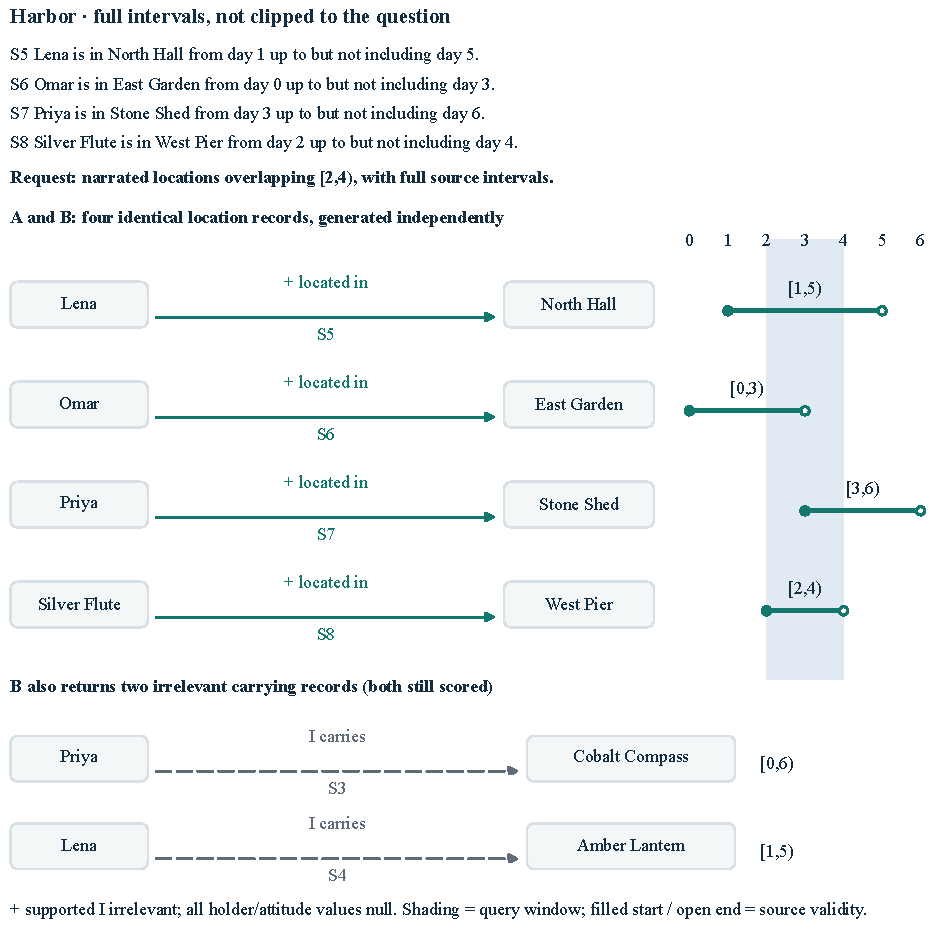
\includegraphics[width=\textwidth]{figures/harbor.pdf}
\caption{Harbor locations from pre-extract/select (A) and contextual extraction (B). Four independently generated records coincide and are shown in aligned rows. B also returns the two carrying edges below. Filled/open circles mark included/excluded bounds. Shading shows the query window, not rewritten validity. Executed question: \HarborQuestion\ Source display S5--S8 from the fourteen sentences supplied to both approaches. All six B predictions remain scored. + indicates supported meaning and I supported but irrelevant content. Holder and attitude are null throughout.}
\label{fig:harbor}
\end{figure*}}
\newcommand{\AliceFigure}{
\begin{figure*}[!t]
\centering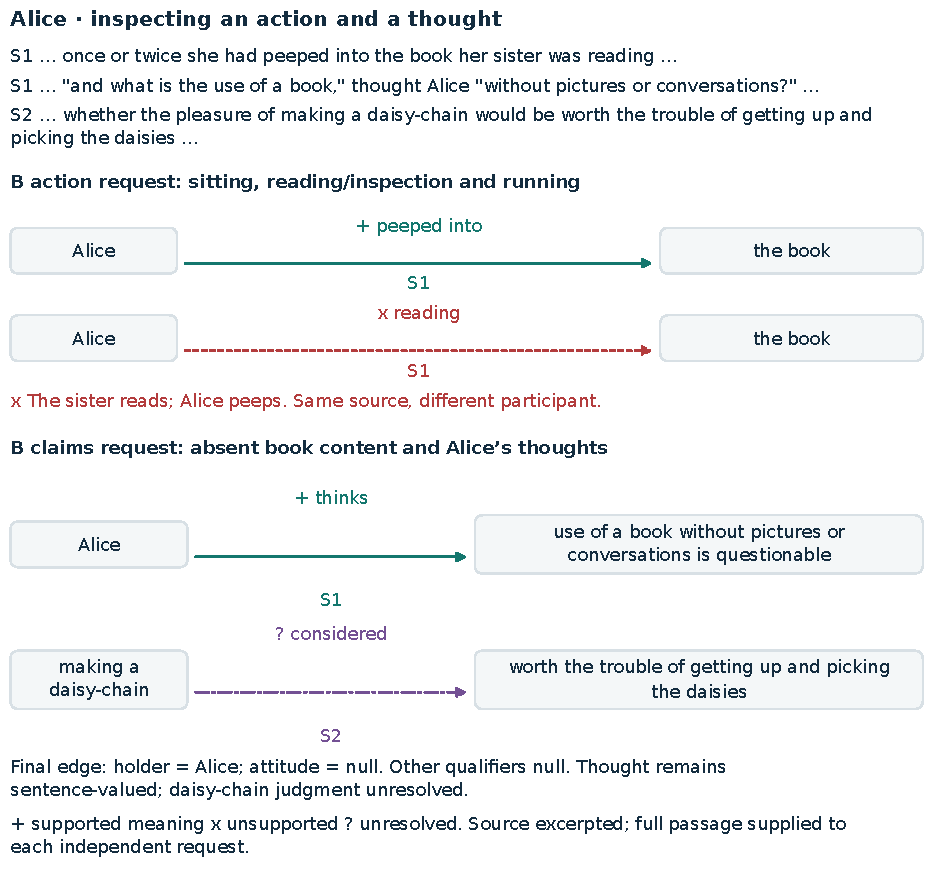
\includegraphics[width=\textwidth]{figures/alice.pdf}
\caption{Alice: independent contextual extraction (B) for two requests over identical complete evidence. Display: two of five action edges (two sitting edges and Rabbit running omitted) and two of three claims (book content omitted). All remain scored. Executed action question: \AliceActionQuestion\ Executed claims question: \AliceClaimQuestion\ Source excerpts are marked. + indicates supported meaning, x an unsupported participant, and ? unresolved consideration. The thought remains the actual sentence-valued object. All bounds are null. The final record has holder Alice and null attitude.}
\label{fig:alice}
\end{figure*}}
